\section{Our Approach}\label{sec:method}
In this section, we present the proposed regularization approach and highlight the  differences between related methods that use adversarial training for regularization. In addition, we perform a small scale experiment to study the properties of the proposed approach by analyzing the singular value spectrum of the Jacobian. We also visualize the impact of these perturbations on the intermediate layer activations and conclude by illustrating the connection to robust optimization-based approaches.

%\subsection*{Notation}
We start by defining some notation. Let $\{x_i\}_{i=1}^{N}$ denote the set of images and $\{y_i\}_{i=1}^{N}$ denote the set of labels. Let $f: x \in \mathbb{R}^{m} \mapsto y \in \mathbb{L}$ denote the classifier mapping that maps the image to a discrete label set, $\mathbb{L}$. In this work, $f$ is modeled by a deep CNN unless specified otherwise. We denote the loss function of the deep network by $\mathcal{J}(\theta,x,y)$ where $\theta$ represents the network parameters and $\{x,y\}$ are the input and output respectively. The deep network consists of $L$ layers and $\nabla_{l}\mathcal{J}(\theta^{t},x^{t},y^{t})$ denotes the backpropagated gradient of the loss function at the output of the ${l}^{th}$ layer at iteration $t$. In the above expression, $l=0$ corresponds to the input layer and $l=L-1$, the loss layer. Let $x^{t}_{l}$ be the input activation to the $l^{th}$ layer and $r^{t}_{l}$ represents the perturbation that is added to $x^{t}_{l}$. For clarity, we drop the subscript $l$ when talking about the input layer. %Update this as required...

\subsection{Overview of Adversarial training methods}
Previous works on adversarial training have observed that training the model with adversarial examples acts as a regularizer and improves the performance of the base network on the test data. \citeauthor{szegedy2013intriguing} \shortcite{szegedy2013intriguing} define adversarial perturbations $r$ as a solution of a box-constrained optimization as follows: Given an input $x$ and target label $y$, they intend to minimize $||r||_{2}$ subject to (1) $f(x+r)=y$ and (2) $x+r \in [0,1]^{m}$. Note that, if $f(x)=y$, then the optimization is trivial (i.e. $r=0$), hence $f(x)\neq y$.  While the exact minimizer is not unique, they approximate it using a box-constrained L-BFGS. More concretely, the value of $c$ is found using line-search for which the minimizer of the following problem satisfies $f(x+r)=\hat{y}$, where $\hat{y}\neq y$:
\begin{equation}
\underset{r}{\text{argmin}} \;  c||r||_{2} + \mathcal{J}(\theta,x+r,y), \quad \text{subject to} \quad x + r \in [0,1]^{m}
\label{eq:lbfgs}
\end{equation}
This can be interpreted as finding a perturbed image $x+r$ that is closest to $x$ and is misclassified by $f$. The training procedure for the above framework involves optimizing each layer by using a pool of adversarial examples generated from previous layers. As a training procedure, this is rather cumbersome even when applied to shallow networks having 5-10 layers. To overcome the computational overhead due to the L-BFGS optimization performed at each intermediate layer, \cite{goodfellow2014explaining} propose the Fast Gradient Sign (FGS) method to generate adversarial examples. By linearizing the cost function around the value of the model parameters at a given iteration, they obtain a norm constrained perturbation as follows: $r_{fgs}=\epsilon . sign(\nabla\mathcal{J}(\theta,x,y))$. They show that the perturbed images $x+r_{fgs}$ reliably cause deep models to misclassify their inputs. As noted in \cite{understandingAT}, the above formulation for adversarial perturbation can be understood by looking at a first order approximation of the loss function $\mathcal{J}(\cdot)$ in the neighborhood of the training sample $x$:

\begin{equation}
\tilde{\mathcal{J}}(\theta,x+r,y) = \mathcal{J}(\theta,x,y)+ \langle \nabla\mathcal{J}(\theta,x,y),r\rangle
\end{equation}

The FGS solution ($r_{fgs}$) is the result of maximizing the second term with respect to $r$, with a $l_{\infty}$ norm constraint. They train the network with the following objective function with an added adversarial objective:
\begin{equation}
\tilde{\mathcal{J}}(\theta,x,y) = \alpha \mathcal{J}(\theta,x,y)+ (1-\alpha) \mathcal{J}(\theta,x+r_{fgs},y)
\label{eq:fgs_train}
\end{equation}


By training the model with both original inputs and adversarially perturbed inputs, the objective function in \ref{eq:fgs_train} makes the model more robust to adversaries and provides marginal improvement in performance on the original test data. Intuitively, the FGS procedure can be understood as perturbing each training sample within a $L_{\infty}$ ball of radius $\epsilon$, in the direction that maximally increases the classification loss. 

% While these gradient directions are guaranteed to be adversarial, training with such adversarial examples do not impose better classifier discriminability. An ideal training framework would not only improve adversarial robustness but also improve the discriminability of the learned classifier mapping. for the  directions are not guaranteed to be the most confusing directions that when used for training would increase the discriminability of the classifier in addition to making it more robust. Furthermore, \cite{goodfellow2014explaining} note that they could not successfully train networks by perturbing the intermediate layers due to unbounded layer activations.

The focus of the adversarial training techniques described above is to improve a model's robustness to adversarial examples. As a by-product, they observe that an adversarial loss term can also marginally regularize the deep network training. In this work, we propose a novel approach which is an extension of the traditional adversarial training. The focus of our approach is to improve regularization and as an interesting by-product, we observe improvement in adversarial robustness of the trained model as well.

\subsection{Proposed Formulation}\label{subsec:formulation}
The proposed approach differs in the following aspects compared to the formulations discussed above: (1) Generating adversarial perturbations from intermediate layers rather than just using the input layer (2) Using the gradients from the previous batch to generate adversarial perturbations for the activations of the current batch. In order to facilitate the representation of layerwise activations in the loss function, we denote the collection of layerwise responses as $X=\{x_l\}_{l=0}^{L-1}$ and  the set of layerwise perturbations as $R=\{r_l\}_{l=0}^{L-1}$. Then, $\mathcal{J}(\theta,X+R,y)$ denotes the loss function where intermediate layer activations are perturbed according to the set $R$. The notation used in the previous section is a special case where $X={x}$ and $R=r_{fgs}$. Now, consider the following objective to obtain the perturbation set $R$: 
%we propose to solve a variant of the above problem that generates adversarial perturbations using samples from different classes in the training set.
\begin{equation}
\begin{aligned}
& \underset{R}{\text{argmax}} \; \mathcal{J}(\theta,X+R,y) \\
& \text{subject to} \quad ||r_{l}||_{\infty} \leq \epsilon, \; \forall l, \; f(X+R) \neq y
\label{eq:our_train}
\end{aligned}
\end{equation}

Ideally, for each training example $x$, the solution to the above problem, consists of generating the perturbation corresponding to the maximally confusing class; in other words, by choosing the class $\hat{y}$ which maximizes the divergence, $KL(p(y|x_{L-1}),p(\hat{y}|x_{L-1}))$.  In the absence of any prior knowledge about class cooccurences, solving this explicitly for each training sample for every iteration is time consuming. Hence we propose an approximate solution to this problem: the gradients computed from the previous sample at each intermediate layer are cached and used to perturb the activations of the current sample. In a mini-batch setting, this amounts to caching the gradients of the previous mini-batch. To ensure the class constraint in Eq. \ref{eq:our_train} is satisfied, the only requirement is that successive batches have little lateral overlap in terms of class labels. From our experiments, we observed that any random shuffle of the data satisfies this requirement. For more discussion on this, please refer to the experiments section. Given this procedure of accumulating gradients, we are no longer required to perform an extra gradient descent-ascent step as in the FGS method to generate perturbations for the current batch. Since the gradient accumulation procedure does not add to the computational cost during training, this can be seamlessly integrated into any existing supervised training procedure including even very deep networks as shown in the experiments. 

\begin{algorithm*}[!htb]
\caption{Efficient layerwise adversarial training procedure for improved regularization}\label{alg:algo}
\label{tab:algo}
\begin{algorithmic}[1]
\State Inputs: Deep network $f$ with loss function $\mathcal{J}$ and parameters $\theta$ containing C convolutional blocks. ${B^t}$ is the batch sampled at iteration $t$ of size $k$, with input-output pairs $\{X^{t},Y^{t}\}$. Gradient accumulation layers $\{G_c\}_{c=1}^{C}$, with stored perturbations $R^t=\{r^{t}_c\}_{c=1}^{C}$, initialized with zero. Perturbation parameter, $\epsilon$.
\State {t=0:}
		\State Sample a batch $\{X^t,Y^t\}$ of size $k$ images from the training data
        \State Perform regular forward pass - $G_c$'s are not active for $t=0$.
        \State Perform backward pass using the classification loss function. Each gradient accumulation layer $G_{c}$ stores the gradient signal backpropagated to that layer:
        \begin{equation}
        r^{t+1}_c = sign(\nabla_{c}\mathcal{J}(\theta^t,X^t+R^t,Y^t)),  \forall c = [1,C]
        \label{eq:update}
        \end{equation}
\For{t in 1:$|B|-1$}
		
		\State Sample a batch $\{X^t,Y^t\}$ of size $k$ from the training data
        \State Perform forward pass with perturbation: Each gradient accumulation layer acts as follows. \noindent Let $X^{t}_{c}$ be the input to block $c$, then:
        \begin{equation}
        		G_c(X^{t}_{c})=X^{t}_{c}+\epsilon \cdot r^{t}_c
         \end{equation}
        \State Perform backward pass updating $r^{t}_c$ to $r^{t+1}_c$ for all blocks $c$ as in Eq. ~\ref{eq:update} above.
\EndFor
\State \textbf{Test time usage:} During test time, the gradient accumulation layers ($G_c$) are removed and $f$ behaves as a standard feed forward deep network.
\end{algorithmic}
\end{algorithm*}

%  Since we are using the gradients from a different image to perturb the given image, we found that the accumulated gradients are not adversarial at the input layer. Furthermore, since our focus is in perturbing the feature space learned by the deep network, we perturb only the intermediate layer activations similar to the work of \cite{szegedy2013intriguing}.
 The training procedure is summarized in Algorithm \ref{tab:algo}, where $sign(\cdot)$ denotes the signum function. We add the gradient accumulation layers after the Batch Normalization layer in each convolutional block (conv-BN-relu). In case BN layers are not present, we add gradient accumulation layers after each convolution layer. A subtle detail that is overlooked in the algorithm is that the value of $\epsilon$ is not constant over all the layers, rather it is normalized by multiplying with the range of the gradients generated at the respective layers. During test time, the gradient accumulation layers ($G_c$) are removed from the trained model.
 
  %Since the output activations of the  batch normalization layer are well bounded, this controls the norm of the perturbations so that they do not explode. This unstable behavior was noted in  \cite{goodfellow2014explaining}, which was one of the reasons they could not successfully train networks by perturbing the intermediate layers. 

To understand the effect of the the proposed layerwise perturbations described in the previous section, we compare them with random layerwise perturbations. Figure \ref{fig:adv_tsne} shows a two dimensional t-SNE \cite{maaten2008visualizing} visualization of the embeddings belonging to the penultimate FC-layer for a range of values of $\epsilon$, the intensity of the adversarial perturbation. 
%they could not successfully train networks by perturbing the intermediate layers
We used a pretrained VGG network that was trained on the CIFAR-10 dataset to compute the embeddings for two randomly chosen classes from the test data. In the bottom row, the effect of random perturbations with zero mean and unit standard deviation, applied layerwise on the original data is also shown. From the visualization and the accuracy values, it can clearly be observed that the proposed perturbations when added to the original data makes the network misclassify the original data. Hence training using these perturbations results in good regularization and improved robustness. Notice that even for higher values of $\epsilon$, the data perturbed by layerwise random gradient directions remains clearly linearly separable while the data perturbed by the accumulated gradients is unable to be distinguished by the base model. 

% \begin{figure*}
% \subfloat[]{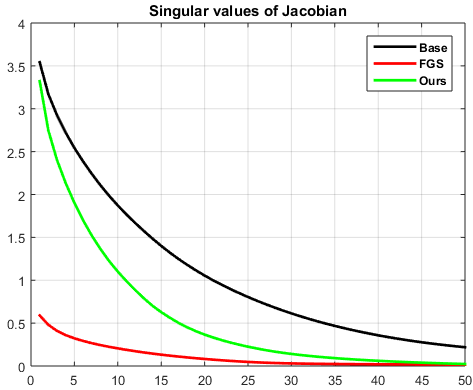
\includegraphics[width=0.5\textwidth]{svalue_jacobian.png}\label{fig:jacobian}}
%   \hfill
%   \subfloat[]{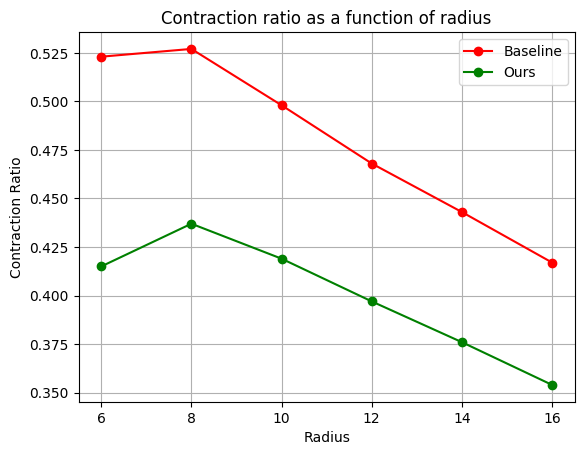
\includegraphics[width=0.5\textwidth]{contractive_radius.png}\label{fig:cradius}}
%   \hfill
% \caption{Average singular value spectrum for the toy example in Section \ref{subsec:toy_eg}. Please refer to the text for details.}
% \end{figure*}

% \begin{figure}
% \begin{floatrow}
% \ffigbox[5cm]{%
%   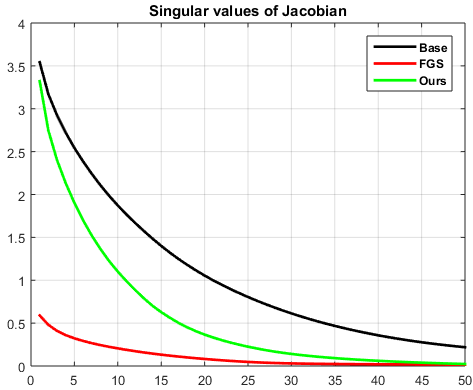
\includegraphics[width=0.4\textwidth]{svalue_jacobian.png}%
% }{%
%   \caption{Average singular value spectrum showing top 50 singular values for the toy example in Section \ref{subsec:toy-eg}. Please refer to the text for details.}%
%  \label{fig:jacobian}
% }
% \capbtabbox[9cm]{%
% \begin{tabular}{|| c | c | c | c | c ||} \cline{2-4}
% \multicolumn{1}{c}{} & \multicolumn{3}{|c|}{FGS perturbation from:}\\ \cline{1-4}
% $\epsilon$ & Baseline n/w & FGS n/w & Our n/w  & \\  \cline{1-5}
% 0.0  & 39.51 & 39.51 & 39.51 &  \multirow{5}{*}{\parbox{0.01\textwidth}{\rotatebox[origin=c]{270}{\small{Baseline n/w}}}} \\  \cline{1-4}
% 0.02  & 8.6 & 32.14 & 26.92 &  \\   \cline{1-4}
% 0.04  & 1.92 & 26.08 & 18.16 &  \\   \cline{1-4}
% 0.06  & 0.51 & 20.74 & 12.23 &  \\   \cline{1-4}
% 0.08  & 0.12 & 16.23 & 8.63 &  \\   \cline{1-4}
% 0.1  & 0.03  & 12.47 & 6.05 &  \\   \hline
%  \end{tabular}
% }
% {%
%   \caption{Original and Adversarial performance comparison for the toy example in Section \ref{subsec:toy-eg}}%
%   \label{tab:toy-adv}
% }
% \end{floatrow}
% \vspace{-5mm}
% \end{figure}

%\begin{tabular}{|rc|c|c|c}
%&&\multicolumn{3}{|c|}{Model to %generate Aversarial Examples}\\ && Baseline&FGS&Ours\\
%&$\epsilon$


%  \begin{tabular}{||c | c | c | c ||}  \hline
%  $\epsilon$ & Baseline & FGS & Ours \\  \hline
%  0.0  & 39.51 & 40.55 & 43.27  \\   \hline
%  0.02  & 8.6 & 38.47 & 38.87 \\   \hline
%  0.04  & 1.92 & 37.44 & 34.56 \\   \hline
%  0.06  & 0.51 & 36.47 & 30.44 \\   \hline
%  0.08  & 0.12 & 35.55 & 26.71 \\   \hline
%  0.1  & 0.03  & 34.64 & 23.63 \\   \hline
%  \end{tabular}
% }{%
%   \caption{Original and Adversarial performance comparison for the toy example in Section \ref{subsec:toy-eg}}%
%   \label{tab:toy-adv}
% }

%  \begin{longtable}[c]{|c|cc|c|c|c|c|}
% \cline{4-7}
% \multicolumn{2}{c}{}& & \multicolumn{4}{c|}{Var Y} \\ 
% \cline{4-7}
% \multicolumn{2}{c}{}& & 
% \rotatebox{90}{Cat Y1\ }&
% \rotatebox{90}{Cat Y2\ }&
% \rotatebox{90}{Cat Y3\ }&
% \rotatebox{90}{Cat Y4\ }\\
%     \hline \multirow{6}{*}{\begin{sideways}Var X\end{sideways}} &   
% \multicolumn{1}{|c}{\multirow{2}{*}{Cat X1}} &
% \multicolumn{1}{c|}{N} & 4 &  &  &  \\
%     \multicolumn{1}{|c|}{}        &                &  
% \multicolumn{1}{c|}{\%} & 100.00\% &  &  & \\
%     \cline{2-7} &
% \multicolumn{1}{|c}{\multirow{2}{*}{Cat X2}} &
% \multicolumn{1}{c|}{N} &  & 7 & 3 &    \\
%    \multicolumn{1}{|c|}{}        &                &  
% \multicolumn{1}{c|}{\%}&  & 70.00\% & 30.00\% &  \\
%     \cline{2-7} &
% \multicolumn{1}{|c}{\multirow{2}{*}{Cat X3}} &
% \multicolumn{1}{c|}{N} &  & 25 &  & 10 \\
%     \multicolumn{1}{|c|}{}        &                &  
% \multicolumn{1}{c|}{\%}&  & 71.43\% &  & 28.57\% \\
%     \hline
% \multicolumn{2}{|c}{\multirow{2}{*}{Total}} &
% \multicolumn{1}{c|}{N} & 4 & 23 & 3 & 10    \\
%     \multicolumn{2}{|c}{}                 &  
% \multicolumn{1}{c|}{\%}& 10.00\% & 57.50\% & 7.50\% & 2.50\% \\
%    \hline
% \end{longtable}

% \begin{figure}
% \centering
% 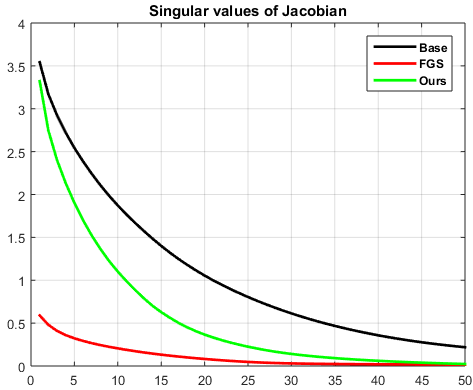
\includegraphics[scale=0.5]{svalue_jacobian.png}
% \caption{Average singular value spectrum for the toy example in Section
% \ref{subsec:toy_eg}. Please refer to the text for details.}
% \label{fig:jacobian}
% \end{figure}
% \hfill
% \begin{center}
% \captionof{table}{Original and Adversarial performance comparison for the toy example in Section \ref{subsec:toy_eg}}
% \label{tab:toy_eg_adv}
%  \begin{tabular}{||c | c | c ||} 
%  \hline
%  Type & Baseline & Perturbed \\ [0.5ex] 
%  \hline
%  VGG  & 92.1 $\pm$ 0.3 & 92.65 $\pm$ 0.2 \\ 
%  \hline
%  Resnet-20 & 90.27 $\pm$ 0.4 & 91.1 $\pm$ 0.3 \\
%  \hline  
%  Resnet-56 & 91.53	$\pm$ 0.3 & 94.1 $\pm$ 0.2 \\
%  \hline 
% \end{tabular}
% \end{center}

\subsection{Toy example}\label{subsec:toy-eg}
In order to acquire a better understanding of the regularizing properties of the mapping function learned using the proposed approach, we perform a toy experiment using a small neural network consisting of two fully connected layers of sizes 1024 and 512. Each fully connected layer is followed by a hyperbolic tangent activations. We use the grayscale version of the CIFAR-10 dataset as our testbed and $L_2$ norm weight decay was applied during training. No data augmentation or other regularization methods such as dropout were used during training. We train three networks: a baseline network, a network with the gradient accumulation layers (as in Algorithm 1) added after each fully connected layer and a network using the FGS training approach. Cross entropy loss was used to train all the networks. In terms of classification accuracy, the proposed method improves the baseline performance from 39.5\% to 43.3\% on the original data while the accuracy of the FGS network is 40.5\%. 

\textbf{Singular Value Analysis:} To gain a deeper understanding of the encoder mapping learned by each network, we perform an analysis similar to \cite{rifai2011contractive} by computing the singular values of the Jacobian of the encoder. Since this is a small architecture, we are able to explicitly compute the Jacobian for each sample in the test set. The average singular value spectrum of the Jacobian for the test data is shown in Figure \ref{fig:jacobian}. We can make the following observations: (a) The singular value spectrum computed for ours and FGS approach has fewer dominant singular values and decays at a much faster rate compared to base network (b) The FGS training suppresses the response of the network strongly in all the dimensions while our approach achieves a strong suppression only for trailing dimensions. This implies that our network is able to better capture data variations that are relevant for classifying original test data hence providing improved performance. On the other hand, FGS achieves slightly improved robustness against adversarial examples compared to our approach by suppressing the network's response strongly even in leading dimensions, as demonstrated in our ablative experiments in the next section. 

\begin{figure}[h!]
\vspace{-1mm}
\centering
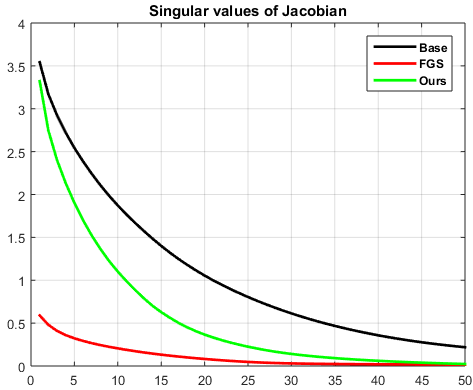
\includegraphics[width=0.3\textwidth, height=0.4\linewidth]{svalue_jacobian.png}
\caption{Average singular value (SV) spectrum showing top 50 SVs for the toy example presented in the text. A model regularized with the proposed approach is compared with a FGS regularized model and baseline model with no regularization.}
\label{fig:jacobian}
\vspace{-3mm}
\end{figure}

% \begin{center}
% \vspace{-6mm}
% \begin{minipage}[t]{.25\linewidth}
% \begin{figure}[H]
% \centering
% 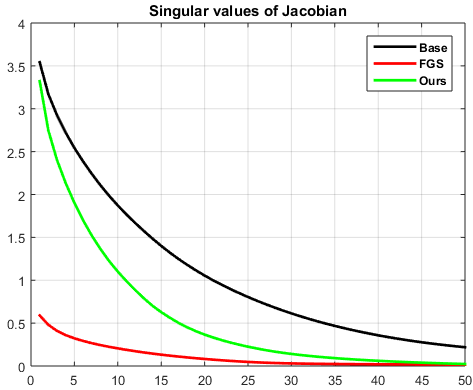
\includegraphics[width=\textwidth]{svalue_jacobian.png}
% \caption{Average singular value (SV) spectrum showing top 50 SVs for the toy example in Section \ref{subsec:toy-eg}.}
% \label{fig:jacobian}
% \end{figure}
% \end{minipage}\hfill
% \begin{minipage}[t]{.25\linewidth}
% \vspace{20pt}
% \begin{table}[H]
% \centering
%  \begin{tabular}{|| c | c | c | c | c ||} \cline{2-4}
% \multicolumn{1}{c}{} & \multicolumn{3}{|c|}{FGS perturbation from:}\\ \cline{1-4}
% $\epsilon$ & Baseline n/w & FGS n/w & Our n/w  & \\  \cline{1-5}
% 0.0  & 39.51 & 39.51 & 39.51 &  \multirow{5}{*}{\parbox{0.01\textwidth}{\rotatebox[origin=c]{270}{\small{Baseline n/w}}}} \\  \cline{1-4}
% 0.02  & 8.6 & 32.14 & 26.92 &  \\   \cline{1-4}
% 0.04  & 1.92 & 26.08 & 18.16 &  \\   \cline{1-4}
% 0.06  & 0.51 & 20.74 & 12.23 &  \\   \cline{1-4}
% 0.08  & 0.12 & 16.23 & 8.63 &  \\   \cline{1-4}
% 0.1  & 0.03  & 12.47 & 6.05 &  \\   \hline
%  \end{tabular}
% \caption{Effect of different perturbations tested on the baseline network for the toy example in Section \ref{subsec:toy-eg}.}
% \label{tab:toy-adv}
% \end{table}
% \end{minipage}
% \end{center}


% \textbf{Degree of ``adversarialness'':} In order to validate this implication, we perform an empirical experiment on the CIFAR-10 test dataset. Each test image is used to generate FGS perturbations using each of the three networks trained above. All the three perturbed images are classified by the baseline network. This process is repeated for all 10,000 images from the test set. Table \ref{tab:toy-adv} lists the performance of the baseline network on the perturbed images for various values of $\epsilon$, the intensity of the FGS perturbation. Intuitively, this experiment characterizes the relative strengths of adversarial examples generated from the three networks mentioned above. To that end, we can observe that the robustness of the base network to different adversarial examples occur in the following order: FGS $>$ Ours $>>$ base. This concurs with the singular value spectrum analysis presented above that the stronger the suppression of the network's response the less sensitive it becomes to adversarial directions. 
% \begin{table}
% \centering
%  \begin{tabular}{|| c | c | c | c | c ||} \cline{2-4}
% \multicolumn{1}{c}{} & \multicolumn{3}{|c|}{FGS perturbation from:}\\ \cline{1-4}
% $\epsilon$ & Baseline n/w & FGS n/w & Our n/w  & \\  \cline{1-5}
% 0.0  & 39.51 & 39.51 & 39.51 &  \multirow{5}{*}{\parbox{0.01\textwidth}{\rotatebox[origin=c]{270}{\small{Baseline n/w}}}} \\  \cline{1-4}
% 0.02  & 8.6 & 32.14 & 26.92 &  \\   \cline{1-4}
% 0.04  & 1.92 & 26.08 & 18.16 &  \\   \cline{1-4}
% 0.06  & 0.51 & 20.74 & 12.23 &  \\   \cline{1-4}
% 0.08  & 0.12 & 16.23 & 8.63 &  \\   \cline{1-4}
% 0.1  & 0.03  & 12.47 & 6.05 &  \\   \hline
%  \end{tabular}
% \caption{Effect of different perturbations tested on the baseline network for the toy example in Section \ref{subsec:toy-eg}.}
% \label{tab:toy-adv}
% \end{table}

% This shows that the ability of the networks to generate adversarial perturbations is related to the singular value spectrum of the Jacobian as follows: strong suppression of the network's response to perturbations deters significantly its own ability to generate adversarial gradients.



% From a model selection perspective, FGS selects a model that suppresses the network's response against perturbations in almost all dimensions thereby providing robustness against adversarial examples. On the other hand, our approach preserves networks capacity to model data variations achieves a non-uniform suppression of singular values which improves the performance on the original test data while marginally decreasing performance on adversarial examples.

% In our case, the leading singular values are still dominant and the spectrum becomes similar to the FGS network at later dimensions. FGS approach achieves a stronger performance on adversarial data by suppressing even the leading dimensions. The proposed approach achieves superior performance on the original data by retaining enough information that help in classification while developing robustness to spurious perturbations by suppressing later dimensions. These empirical results are shown in Table \ref{tab:toy-adv}. A similar effect is presented along with a more detailed discussion for a much deeper network in Section \ref{subsec:variants}.

% This implies that the proposed learning method is able to capture only those variations of the training data required for better classification performance. \cite{wang2016theoretical} note that robustness of classifiers to adversarial examples can be improved by suppressing those dimensions that are not useful for the classification objective. Based on recent theoretical findings , this could be a possible explanation as to why our approach provides more robustness on the adversarial test set.  
\begin{figure*}[!h]
  \centering
  \subfloat[$\epsilon=0, 91.9\% $]{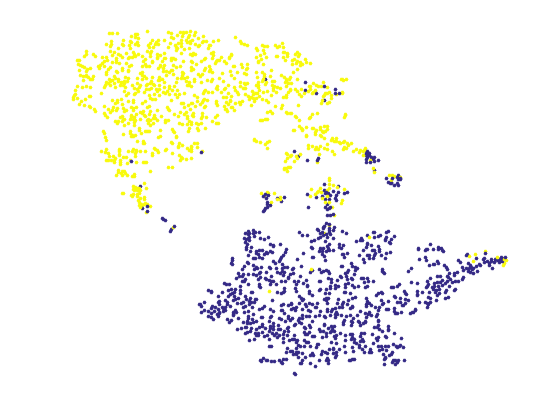
\includegraphics[width=0.24\textwidth,height=0.1\linewidth]{eps_0_0.png}\label{fig:f1}}
  \hfill
  \subfloat[$\epsilon=0.02, 69.4\%$]{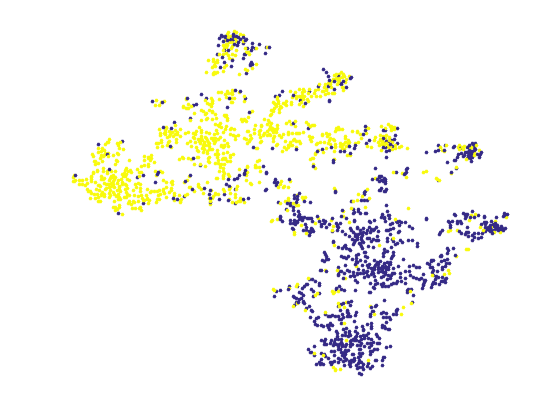
\includegraphics[width=0.24\textwidth,height=0.1\linewidth]{eps_0_02.png}\label{fig:f2}}
  \hfill
  \subfloat[$\epsilon=0.04, 48.2\%$]{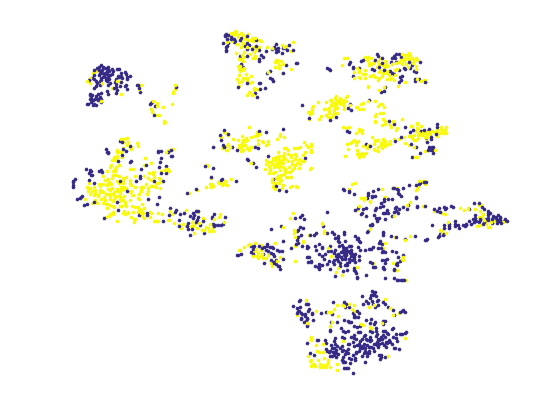
\includegraphics[width=0.24\textwidth,height=0.1\linewidth]{eps_0_04.png}\label{fig:f3}}
  \hfill
  \subfloat[$\epsilon=0.06, 34.6\%$]{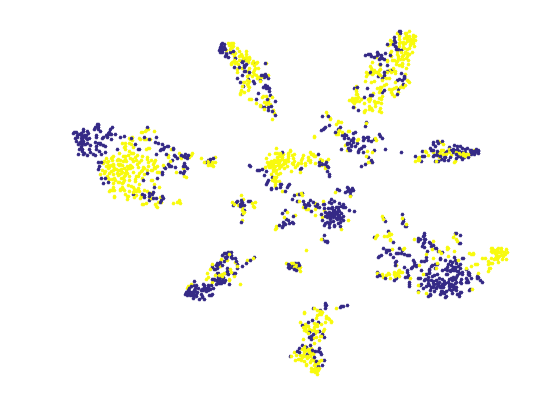
\includegraphics[width=0.24\textwidth,height=0.1\linewidth]{eps_0_06.png}\label{fig:f4}} \\
   
  \subfloat[$\epsilon=0, 91.9\%$]{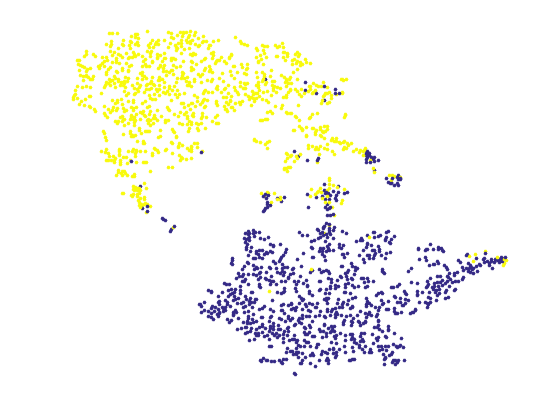
\includegraphics[width=0.24\textwidth,height=0.1\linewidth]{eps_0_0.png}\label{fig:f1}}
  \hfill
  \subfloat[$\epsilon=0.02, 91.85\%$]{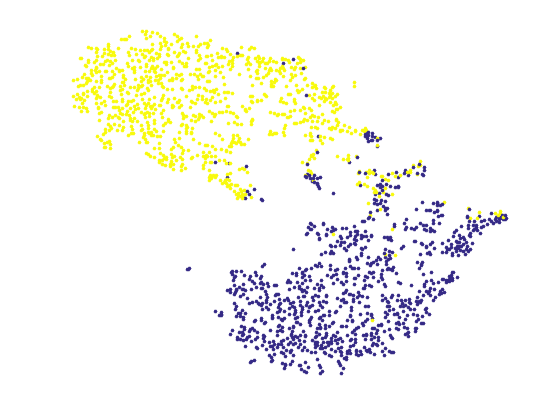
\includegraphics[width=0.24\textwidth,height=0.1\linewidth]{eps_0_02_random.png}\label{fig:f2}}
  \hfill
  \subfloat[$\epsilon=0.04, 91.9\%$]{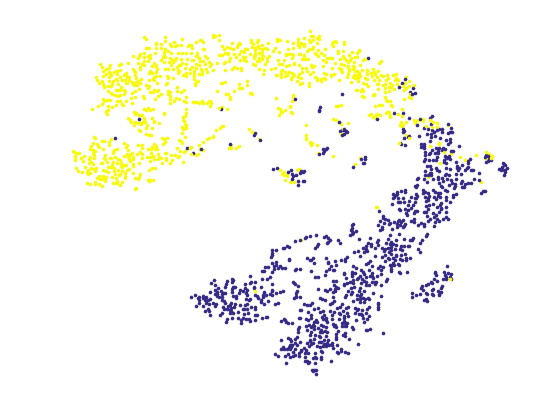
\includegraphics[width=0.24\textwidth,height=0.1\linewidth]{eps_0_04_random.png}\label{fig:f3}}
  \hfill
  \subfloat[$\epsilon=0.06, 85.8\%$]{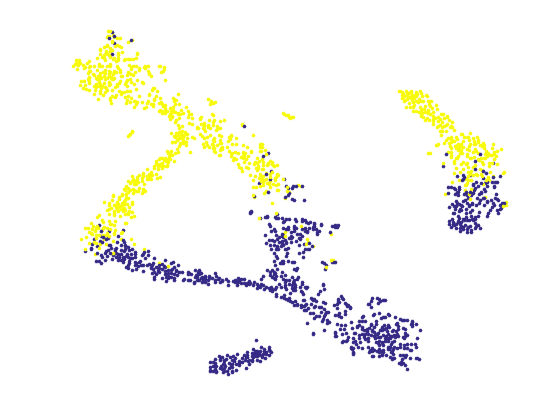
\includegraphics[width=0.24\textwidth,height=0.1\linewidth]{eps_0_06_random.png}\label{fig:f4}}
  \caption{t-SNE visualization of the final fc-layer features of dimension 512 of the VGG network for two randomly chosen classes of the CIFAR-10 data for different values of the intensity, $\epsilon$. The top row shows the effect of the perturbations generated using the proposed approach while the bottom row shows random perturbations of the same intensity. It is clear that the random perturbations do not affect the linear separability of the data, while the proposed perturbations are extremely effective in leading the network to misclassify the perturbed data.}
\label{fig:adv_tsne}
\end{figure*}

\subsection{Connection to Robust Optimization}
Several regularization problems in machine learning such as ridge regression, lasso or robust SVMs have been shown to be instances of a more general robust optimization framework \cite{sra2012optimization}. To point out the connection between the proposed approach and robust optimization, we borrow the idea of uncertainty sets from \cite{understandingAT}. To explain briefly, an uncertainty set denoted by $\mathcal{U} = \mathcal{B}_{\rho}(x,\epsilon)$ represents an epsilon ball around $x$ under norm $\rho$. \cite{goodfellow2014explaining} point out that adversarial training can be thought of as training with hard examples that strongly resist classification. 
%They also perturb the inputs using random noise by an uniform $\epsilon$ ball around each sample and report no difference in original or adversarial performance. 
Under the setting of uncertainty sets, adversarial training with the FGS method could be seen as generating the worst case perturbations from the input space $\mathcal{U}$ under the $l_{\infty}$ norm. In this work, we extend the idea of uncertainty sets from input activations to intermediate layer activations. This can be thought of as sampling perturbations from the feature space learned by the deep network. 
Let $\mathcal{U}_{l}$ represent the uncertainty set of the activation $x_{l}$ at layer $l$. Then, the proposed adversarial training approach is equivalent to sampling perturbations from the intermediate layer uncertainty sets which makes the feature representation learned at those layers to become more robust during training. Moreover, by generating perturbations from inputs that do not belong to the same class as the current input, the directions sampled from the uncertainty set tend to move the perturbed feature representation towards the direction of an adversarial class. This effect can be observed from the t-SNE visualization shown in Figure \ref{fig:adv_tsne}. 




% ******* we should talk about why more adversity is good ****** Is there any theoram which states that or conclusion from another paper. ***** 


% \begin{equation}
% \underset{p,\hat{y} \neq y}\text{minimize}
% \end{equation}
% %c||p||_{2} + \mathcal{J}(\theta,x+p,y') \quad \text{subject to} \quad x + p \in [0,1]^{d}


% From the stand point of adversarial training, the most widely used methods to make the network robust include (1) augmenting the training data with adversarial examples generated from a pretrained model and training a model anew (2) Performing an extra gradient ascent step during training to generate adversarial inputs on the fly for each batch. 


% In this section, we formalize that viewpoint and propose a more efficient way to 

% *** Analyze the perturbations in terms of reliability and compare with fast sign in terms of performance reduction ***

% *** Start with LBFGS box optimization from Szegedy et al and explain fast sign then get into our method ***

% *** Analyze the effect of adding this only to higher layers / lower layers etc ***
% *** whats the rule of thumb for setting epsilon ? ***


% Our method cover the directions of variations that are both adversarial and the natural variations from the training data, suppresses spurious dimensions in the feature space unnecessary for the classification task